\documentclass{standalone}
\usepackage{pgf, tikz}
\usetikzlibrary{arrows, automata, positioning}

\begin{document}

    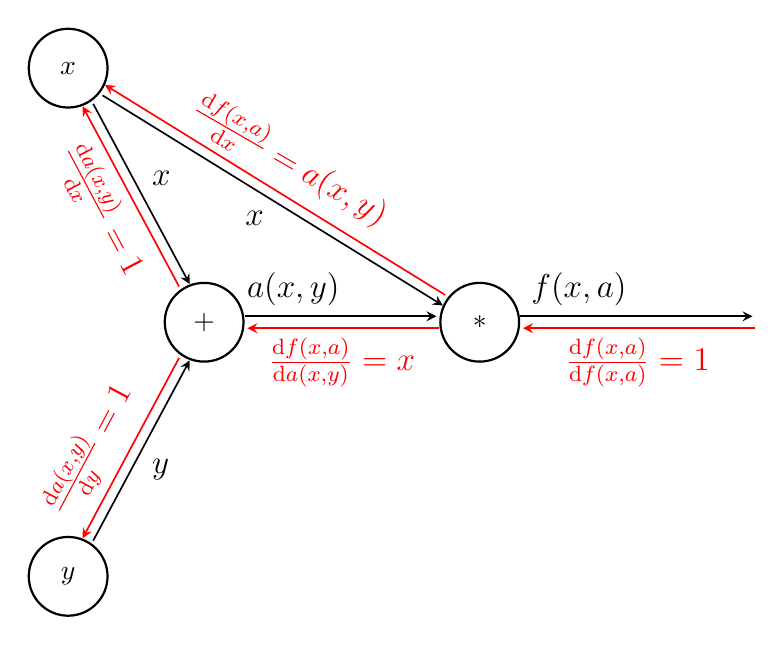
\begin{tikzpicture}[
            > = stealth, 
            shorten > = 1pt, 
            auto,
            node distance = 3.5cm,
            semithick
        ]

        \tikzstyle{every state}=[
            draw = black,
            thick,
            fill = white,
            minimum size = 10mm
        ]
        \tikzset{every edge/.append style={font=\large}}

		\node[state] (add) {$+$};
        \node[state] (x) [above left=2.5cm and 1cm of add] {$x$};
        \node[state] (y) [below left=2.5cm and 1cm of add] {$y$};        
        \node[state] (mul) [right of=add] {$*$};
        \coordinate[right of=mul] (f);
        
        \path[->,transform canvas={xshift=0.5ex}] (x) edge node[above right] {$x$} (add);        
        \path[->,transform canvas={yshift=-0.5ex}] (x) edge node[below left] {$x$} (mul);        
        \path[->,transform canvas={xshift=0.5ex}] (y) edge node[below right] {$y$} (add);        
        \path[->,transform canvas={yshift=0.5ex}] (add) edge node[near start] {$a(x,y)$} (mul);
        \path[->,transform canvas={yshift=0.5ex}] (mul) edge node[near start] {$f(x,a)$} (f);
      
        % partial edges
        \iftrue
        \path[->,transform canvas={xshift=-0.5ex}] (add) edge [red] node[below,  rotate=-62] {$\frac{\mathrm{d}a(x,y)}{\mathrm{d}x} = 1$} (x);
        \path[->,transform canvas={yshift=0.5ex}] (mul) edge [red] node[above, rotate=-30] {$\frac{\mathrm{d}f(x,a)}{\mathrm{d}x} = a(x,y)$} (x);
        \path[->,transform canvas={xshift=-0.5ex}] (add) edge [red] node[above left, rotate=62, pos=0.2] {$\frac{\mathrm{d}a(x,y)}{\mathrm{d}y} = 1$} (y);
        \path[->,transform canvas={yshift=-0.5ex}] (mul) edge [red] node {$\frac{\mathrm{d}f(x,a)}{\mathrm{d}a(x,y)} = x$} (add);
        \path[->,transform canvas={yshift=-0.5ex}] (f) edge [red] node {$\frac{\mathrm{d}f(x,a)}{\mathrm{d}f(x,a)} = 1$} (mul);
        \fi
        

    \end{tikzpicture}

\end{document}